%\documentclass[answers]{exam}
\documentclass{exam}
\usepackage{/Users/nicolasbancel/git/education_suger/mypackages}
\usepackage{/Users/nicolasbancel/git/education_suger/macros}

\SolutionEmphasis{\color{blue}}
\renewcommand{\solutiontitle}{\noindent}

%\usepackage{blindtext}

\renewcommand{\arraystretch}{1.5} % Augmente l'espacement vertical entre les lignes du tableau
\newcolumntype{C}{>{\centering\arraybackslash}m{2cm}}


\SetLabelAlign{myright}{\hss\llap{$#1$}}
\newlist{where}{description}{1}
\setlist[where]{labelwidth=2cm,labelsep=1em,
                        leftmargin=!,align=myright,font=\normalfont}

\setlength{\parindent}{0pt}

\title{Fiche d'exercices corrigée}
\author{N. Bancel}
\date{15 Mai 2025}

\begin{document}


\textbf{Collège Lycée Suger}
\hfill
\textbf{Maths} \\

\textbf{Année 2024-2025}
\hfill
\textbf{1ères STD2A} \par

{\let\newpage\relax\maketitle}
%\maketitle




\section*{Probabilité de Défectuosité d'Aiguilles par Site de Production}

    \begin{figure}[H]
      \centering
      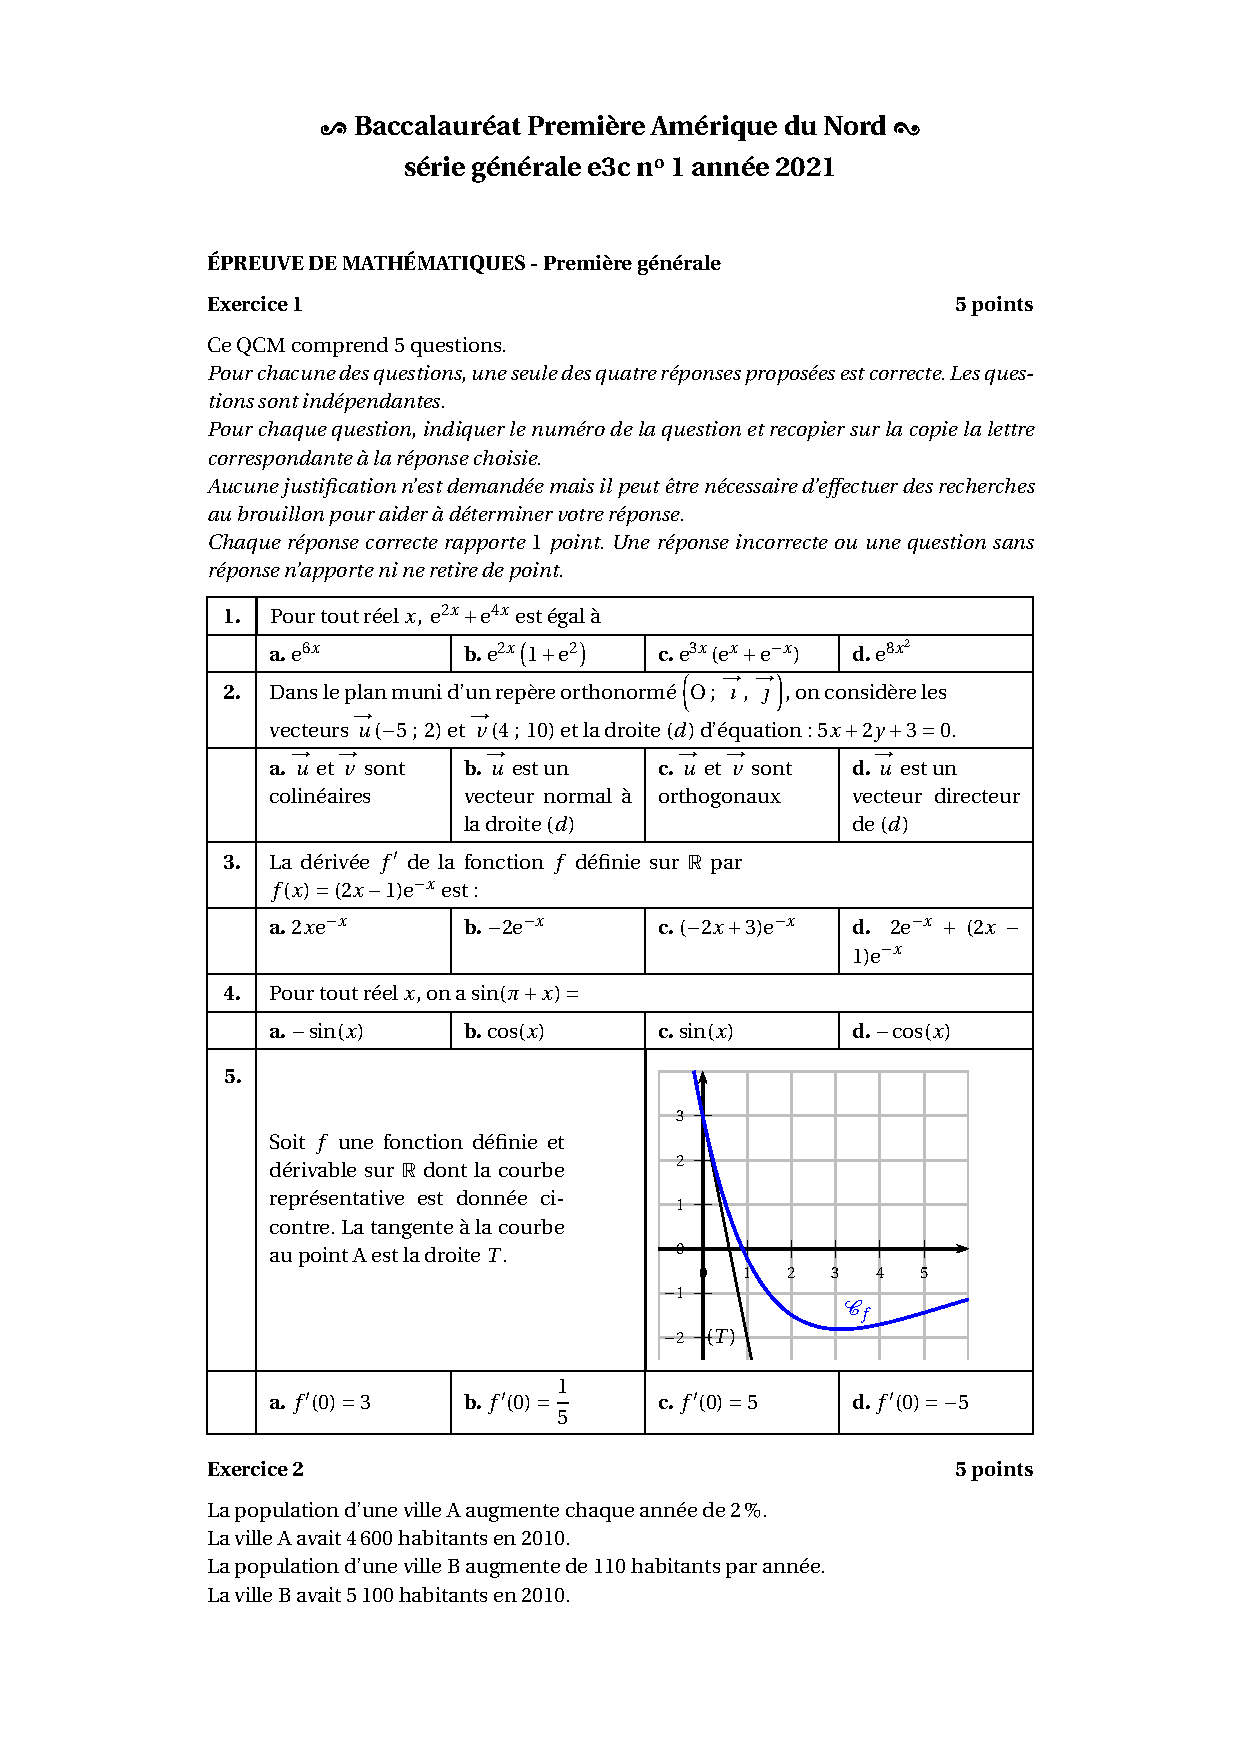
\includegraphics[width=0.6\linewidth]{/Users/nicolasbancel/git/education_suger/00_1ères_STD2A_maths/08_probabilités/fiche_1/e3c_2021_amerique_nord_dv_3.jpg}
      \captionsetup{labelformat=empty}
    \end{figure}

    \begin{solution}

\subsection*{1. Probabilité de l'évènement $A$}

D'après les données de l'énoncé, on sait que le site $A$ produit les trois-quarts des aiguilles. Ainsi, la probabilité que l'aiguille choisie provienne du site $A$ est :
\[
P(A) = \frac{3}{4}
\]

\subsection*{2. Arbre de probabilités}

L'arbre de probabilités se complète de la manière suivante :

\begin{compactitem}
   \item Probabilité que l'aiguille provienne du site $B$: \( P(B) = \frac{1}{4} \)
   \item Probabilité que l'aiguille soit défectueuse et provienne du site $A$: \( P(D|A) = 0,02 \)
   \item Probabilité que l'aiguille ne soit pas défectueuse et provienne du site $A$: \( P(\bar{D}|A) = 1 - 0,02 = 0,98 \)
   \item Probabilité que l'aiguille soit défectueuse et provienne du site $B$: \( P(D|B) = 0,04 \)
   \item Probabilité que l'aiguille ne soit pas défectueuse et provienne du site $B$: \( P(\bar{D}|B) = 1 - 0,04 = 0,96 \)
\end{compactitem}


\subsection*{3. Probabilité que l'aiguille soit défectueuse et provienne du site $A$}

On cherche la probabilité que l'aiguille ait un défaut et provienne du site $A$. Cela se calcule via :
\[
P(D \cap A) = P(A) \times P(D|A)
\]

1. Raisonnement avec formules mathématiques :
   \[
   P(D \cap A) = \frac{3}{4} \times 0,02
   \]

2. Application numérique :
   \[
   P(D \cap A) = 0,015
   \]

\subsection*{4. Montrer que $P(D) = 0,025$}

La probabilité qu'une aiguille ait un défaut est donnée par :
\[
P(D) = P(A) \times P(D|A) + P(B) \times P(D|B)
\]

1. Raisonnement avec formules mathématiques :
   \[
   P(D) = \frac{3}{4} \times 0,02 + \frac{1}{4} \times 0,04
   \]

2. Application numérique :
   \[
   P(D) = 0,015 + 0,01 = 0,025
   \]

3. Conclusion:
   Ainsi, la probabilité qu'une aiguille soit défectueuse est bien de 0,025.

\subsection*{5. Probabilité que l'aiguille ait été produite sur le site $A$ sachant qu'elle est défectueuse}

On cherche \( P(A|D) \), la probabilité que l'aiguille provienne de $A$ sachant qu'elle a un défaut. Cela se calcule via la formule de Bayes :
\[
P(A|D) = \frac{P(D \cap A)}{P(D)}
\]

1. Raisonnement avec formules mathématiques :
   \[
   P(A|D) = \frac{0,015}{0,025}
   \]

2. Application numérique :
   \[
   P(A|D) = 0,6
   \]

3. Conclusion:
   La probabilité que l'aiguille ait été produite sur le site $A$ sachant qu'elle est défectueuse est de 0,6, soit \( \SI{60}{\percent} \).

\end{solution}



\section*{Probabilités conditionnelles avec arbre pondéré}

    \begin{figure}[H]
      \centering
      \includegraphics[width=0.6\linewidth]{/Users/nicolasbancel/git/education_suger/00_1ères_STD2A_maths/08_probabilités/fiche_1/e3c_1ere_2020_serie_2.jpg}
      \captionsetup{labelformat=empty}
    \end{figure}

    \begin{solution}

\subsection*{1. Compléter l'arbre pondéré}

L'arbre pondéré se décompose avec les probabilités suivantes :

\begin{itemize}
  \item \textbf{Noeud S :} 
  \begin{compactitem}
    \item \( P(S) = 0.28 \)
    \item \( P(C|S) = 0.40 \)
    \item \( P(\overline{C}|S) = 0.60 \)
  \end{compactitem}
  \item \textbf{Noeud M :}
  \begin{compactitem}
    \item \( P(M) = 0.42 \)
    \item \( P(C|M) = 0.55 \)
    \item \( P(\overline{C}|M) = 0.45 \)
  \end{compactitem}
  \item \textbf{Noeud J :}
  \begin{compactitem}
    \item \( P(J) = 0.30 \) (par complémentarité)
    \item \( P(C|J) = 0.75 \)
    \item \( P(\overline{C}|J) = 0.25 \)
  \end{compactitem}
\end{itemize}

\subsection*{2. Probabilité qu'une personne ait entre 25 et 60 ans et ne connaisse pas le produit}

Calcul de \( P(M \cap \overline{C}) \).

\begin{align*}
P(M \cap \overline{C}) &= P(M) \cdot P(\overline{C}|M) \\
&= 0.42 \cdot 0.45 \\
&= 0.189
\end{align*}

\subsection*{3.a. Probabilité de l'événement \( S \cap C \)}

Calcul de \( P(S \cap C) \).

\begin{align*}
P(S \cap C) &= P(S) \cdot P(C|S) \\
&= 0.28 \cdot 0.40 \\
&= 0.112
\end{align*}

\subsection*{3.b. Probabilité de l'événement C}

Calcul de \( P(C) \) par la formule de la probabilité totale.

\begin{align*}
P(C) &= P(S \cap C) + P(M \cap C) + P(J \cap C) \\
&= P(S) \cdot P(C|S) + P(M) \cdot P(C|M) + P(J) \cdot P(C|J) \\
&= 0.28 \cdot 0.40 + 0.42 \cdot 0.55 + 0.30 \cdot 0.75 \\
&= 0.112 + 0.231 + 0.225 \\
&= 0.568
\end{align*}

\subsection*{4. Probabilité qu'une personne ait plus de 60 ans sachant qu'elle déclare connaître le produit}

Calcul de \( P(S|C) \).

\[
P(S|C) = \frac{P(S \cap C)}{P(C)} = \frac{0.112}{0.568} \approx 0.197
\]

\textbf{Conclusion:} La probabilité qu'une personne ait plus de 60 ans, sachant qu'elle déclare connaître le produit, est de 0.197.

\end{solution}

\end{document}
